%!TEX root = ../template.tex
%%%%%%%%%%%%%%%%%%%%%%%%%%%%%%%%%%%%%%%%%%%%%%%%%%%%%%%%%%%%%%%%%%%
%% chapter1.tex
%% NOVA thesis document file
%%
%% Chapter with introduction
%%%%%%%%%%%%%%%%%%%%%%%%%%%%%%%%%%%%%%%%%%%%%%%%%%%%%%%%%%%%%%%%%%%

\typeout{NT FILE chapter1.tex}%

\chapter{Introduction}
\label{cha:introduction}

\prependtographicspath{{Chapters/Figures/Covers/}}

% epigraph configuration
\epigraphfontsize{\small\itshape}
\setlength\epigraphwidth{12.5cm}
\setlength\epigraphrule{0pt}


\includegraphics[width=0.1\linewidth]{NOVAthesisFiles/Images/novathesis-insignia}\hfill

\includegraphics[width=0.875\linewidth]{NOVAthesisFiles/Images/novathesis-text}

\epigraph{
  This work is licensed under the \href{https://www.latex-project.org/lppl/lppl-1-3c/}{\LaTeX\ Project Public License v1.3c}.
  To view a copy of this \ntindex[Template!]{license}, visit the \href{https://www.latex-project.org/lppl/}{LaTeX project public license}.
}

\section{Welcome to the \novathesis\ Template}
\label{sec:if_you_use_this_template}

\subsection{Your Time is Precious}
\label{sub:time_is_money}

Did you learn how to drive by sitting by the wheel and throwing your car into the road?  Most probably you did take your time \emph{learning the rules} and \emph{practicing} first! Likewise, it is not wise to throw yourself at the task of writing a thesis/dissertation in \LaTeX\ without seriously considering the following \ntindex{recommendation}!



\subsection{Recognition}
\label{sub:recognition}

\ntindex[Recognition]{}

\section{The \emph{NOVAthesis} Template}
\label{sec:a_bit_of_history}

\ntindex[Template]{}

\newenvironment{ntUniversity}[1]{
  \renewcommand\tabularxcolumn[1]{m{##1}}% for vertical centering text in X column
  % \renewcommand\cellgape{\Gape[1cm]}
  % \setcellgapes{20pt}
  % \makegapedcells
  % % \setlength{\extrarowheight}{20pt}
  % \renewcommand{\arraystretch}{2}
  \rowcolors{1}{}{GhostWhite}
    \xltabular{\linewidth}{cX}%
      \caption{#1's Schools supported by the \gls{novathesis} template\label{tab:supported_schools_#1}}\\
    \toprule%
    \rowcolor{Gainsboro}%
    & \Gape[1.5ex]{\thead[l]{#1}}\\
    \midrule%
}{%
    \bottomrule
    \endxltabular%
}

\makeatletter
\newtoggle{coverspace}
\newcommand{\docCover}[1]{%
  \setlength{\fboxsep}{0pt}%
  \togglefalse{coverspace}%
    \Gape[1.5ex]{\begin{mcellbox}[cc]
    \@for\myi:=#1\do{%
      \fbox{\colorbox{White}{\includegraphics[align=c,width=1.5cm]{1up/\myi}}}%
        \ifx\@xfor@nextelement\@nnil
          % last iteration
        \else
          % not last iteration
          \iftoggle{coverspace}{\togglefalse{coverspace}\\\\[-14pt]}{\toggletrue{coverspace}~}%
        \fi
  }%
    \end{mcellbox}}
}
\makeatother
\newcommand{\schlName}[3]{\textbf{#1} (\href{#3}{#2})}
\newcommand{\degreeName}[3]{\newline\null\quad • #1 \href{#3}{(#2)}}


\newdata*{schlname}
\newdata*{schlurl}
\schlname(ea):={School of Architecture}
\schlurl(ea):={https://www.uminho.pt/EN/uminho/Units/schools-and-institutes/Pages/School-of-Architecture.aspx}
\schlname(ec):={School of Sciences}
\schlurl(ec):={https://www.uminho.pt/EN/uminho/Units/schools-and-institutes/Pages/school-of-sciences.aspx}
\schlname(ed):={School of Law}
\schlurl(ed):={https://www.uminho.pt/EN/uminho/Units/schools-and-institutes/Pages/school-of-law.aspx}
\schlname(ee):={School of Engineering}
\schlurl(ee):={https://www.uminho.pt/EN/uminho/Units/schools-and-institutes/Pages/school-of-Engineering.aspx}
\schlname(eeg):={School of Economics and Management}
\schlurl(eeg):={https://www.uminho.pt/EN/uminho/Units/schools-and-institutes/Pages/school-of-economics-and-management.aspx}
\schlname(em):={School of Medicine}
\schlurl(em):={https://www.uminho.pt/EN/uminho/Units/schools-and-institutes/Pages/school-of-Medicine.aspx}
\schlname(ep):={School of Psychology}
\schlurl(ep):={https://www.uminho.pt/EN/uminho/Units/schools-and-institutes/Pages/school-of-psychology.aspx}
\schlname(ese):={School of Nursing}
\schlurl(ese):={https://www.uminho.pt/EN/uminho/Units/schools-and-institutes/Pages/school-of-nursing.aspx}
\schlname(i3b):={Research Institute 13Bs}
\schlurl(i3b):={https://www.uminho.pt/EN/uminho/Units/schools-and-institutes/Pages/Institute-I3Bs.aspx}
\schlname(ics):={Institute of Social Sciences}
\schlurl(ics):={https://www.uminho.pt/EN/uminho/Units/schools-and-institutes/Pages/institute-of-social-sciences.aspx}
\schlname(ie):={Institute of Education}
\schlurl(ie):={https://www.uminho.pt/EN/uminho/Units/schools-and-institutes/Pages/institute-of-education.aspx}
\schlname(elach):={School of Arts and Humanities}
\schlurl(elach):={https://www.uminho.pt/EN/uminho/Units/schools-and-institutes/Pages/school-of-arts-and-humanities.aspx}



%
% % \begin{ntUniversity}{ISCTE — Instituto Universitário de Lisboa}
% %     \ntSchool{cover-iscteiul-eta-phd}%
% %              {Escola{ de Tecnologias e Arquitectura};{ETA-ISCTE-IUL};{https://ciencia.iscte-iul.pt/schools/escola-tecnologias-arquitectura}%}
% % \end{ntUniversity}
%


\section{Getting Started}
\label{sec:getting_started}

The template provides an \emph{easy to use} setting for you to write your thesis/dissertation in \LaTeX:
\begin{itemize}
  \item  Select your school;
  \item Fill your thesis metadata (title, research field, etc) in the file “\texttt{template.tex}”;
  \item Create your thesis/dissertation contents using the files in folder “\texttt{Chapters}”; and
  \item Process using you favorite \LaTeX\ processor (pdf\LaTeX, \XeLaTeX\ or \LuaLaTeX).
\end{itemize}

\subsection{Using Overleaf}
\label{sub:using_overleaf}

\ntindex[Installation!Overleaf]{}
\ntindex[Using!Overleaf]{}

\newcommand{\Overleaf}{\href{https://www.overleaf.com?r=f5160636&rm=d&rs=b}{Overleaf}}

\begin{wrapfigure}{r}{0.3\linewidth}
% \vspace*{-10ex}
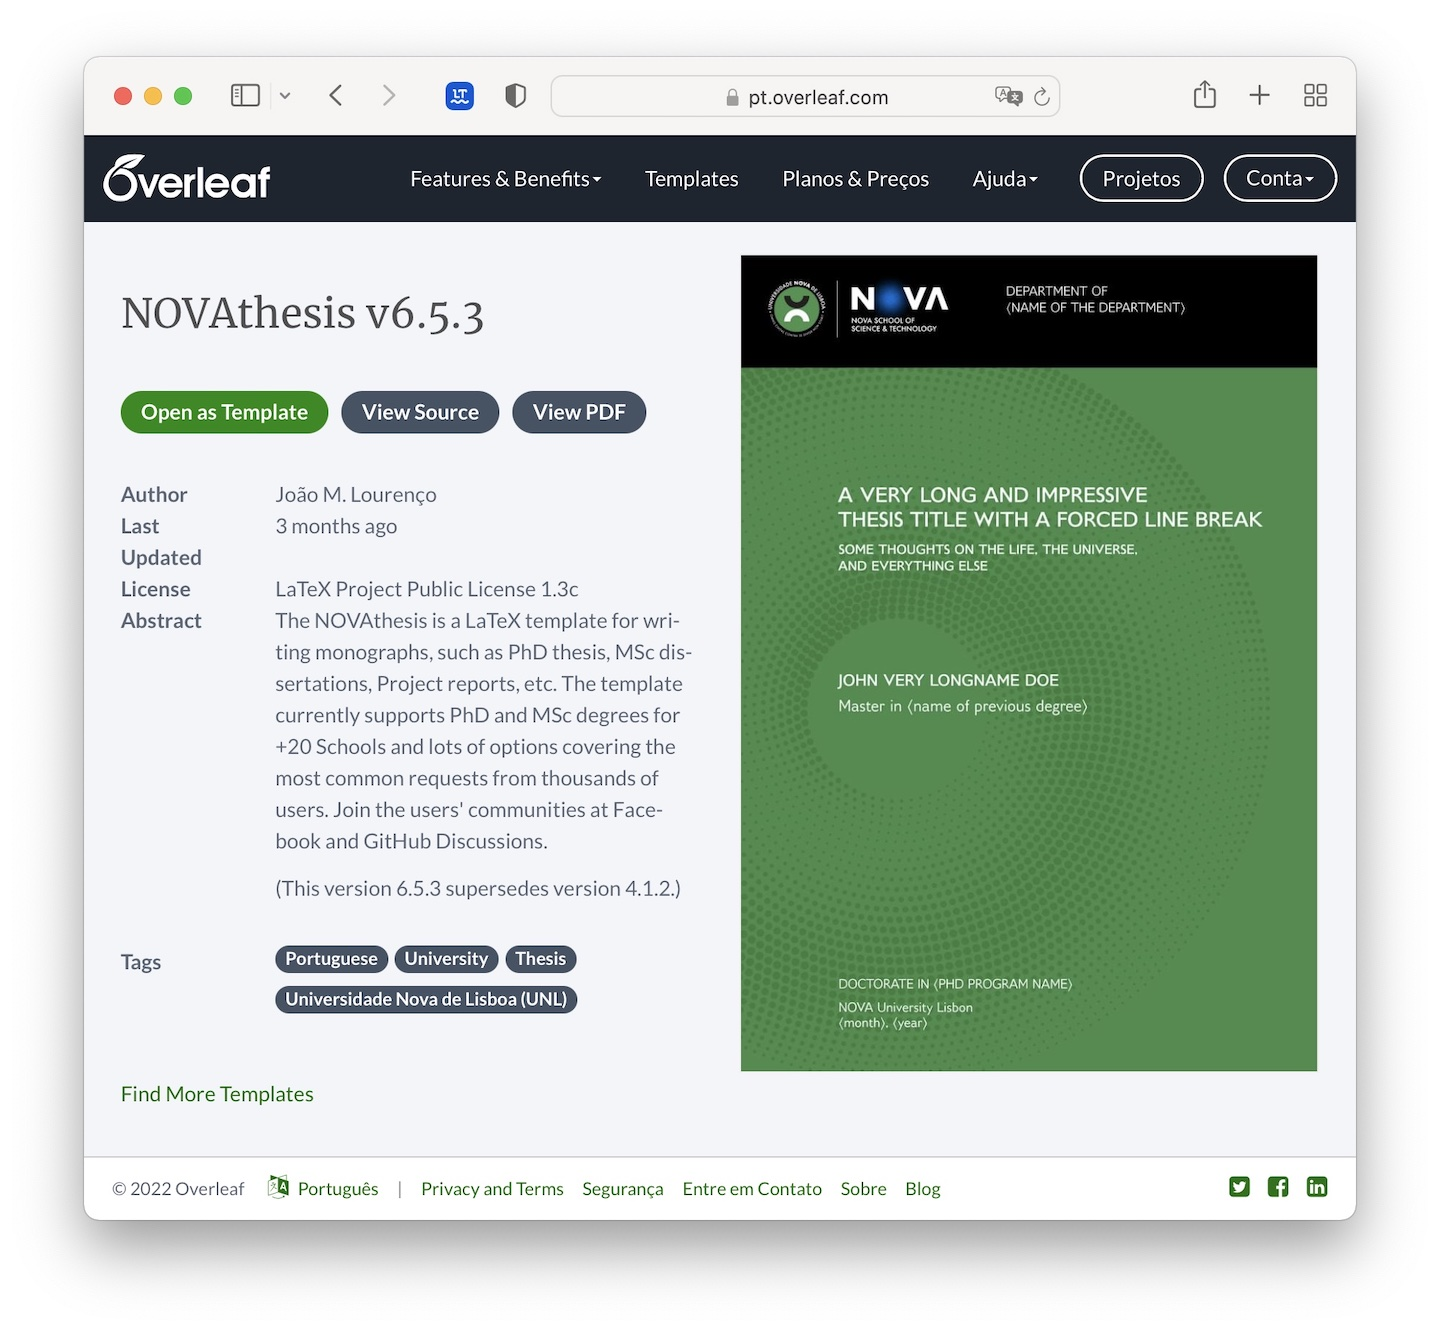
\includegraphics[width=\linewidth]{overleaf}%
\caption{NOVAthesis template in Overleaf.}
\label{fig:overleaf}
\end{wrapfigure}
\mbox{}\Overleaf\ is a collaborative cloud-based LaTeX editor used for writing, editing and publishing scientific documents. Like “Google Docs”,  for \LaTeX\ users. You can edit and compile your \LaTeX\ source on the cloud, without installing software in your own computer, and, much like \emph{Google Docs}, you can share your document with others users and everybody can edit the same file at the same time (this may be dangerous).

If you do not have an account in \Overleaf, you must \href{https://www.overleaf.com?r=f5160636&rm=d&rs=b}{create one first}.


\bgroup
  \itshape
  Please notice that the version currently available in Overleaf (v7.1.18) is slightly outdated (current version is v\novathesisversion). A new version (v7.1.29) will be submitted to Overleaf soon.  Until then, please:
  \begin{enumerate}
    \item Download the \href{https://github.com/joaomlourenco/novathesis/archive/main.zip}{latest version} from the GitHub repository as a Zip file.
    \item Login to your favorite LaTeX cloud service. I recommend \href{https://www.overleaf.com/?r=f5160636&rm=d&rs=b}{Overleaf} but there are alternatives (these instructions apply to Overleaf and you'll have to adapt for other providers).
    \item In the menu select: \texttt{New project} $\rightarrow$ \texttt{Upload project}.
    \item Upload the zip file.
    \item Select “template.tex” as the main file.
    \item Let Overleaf compile the document.
  \end{enumerate}
\egroup

\begin{tcolorbox}[colback=red!8]
	Notice that you need a (student) subscription to compile the \novathesis\ template in Overleaf, otherwise your compilation will always time out.
\end{tcolorbox}

\subsection{Using a Local \LaTeX\ Installation Local}
\label{sub:using_local_latex}

\ntindex[Installation!Local installation]{}
\ntindex[Using!Local installation]{}

\begin{wrapfigure}{r}{0.3\linewidth}
\vspace*{-7ex}
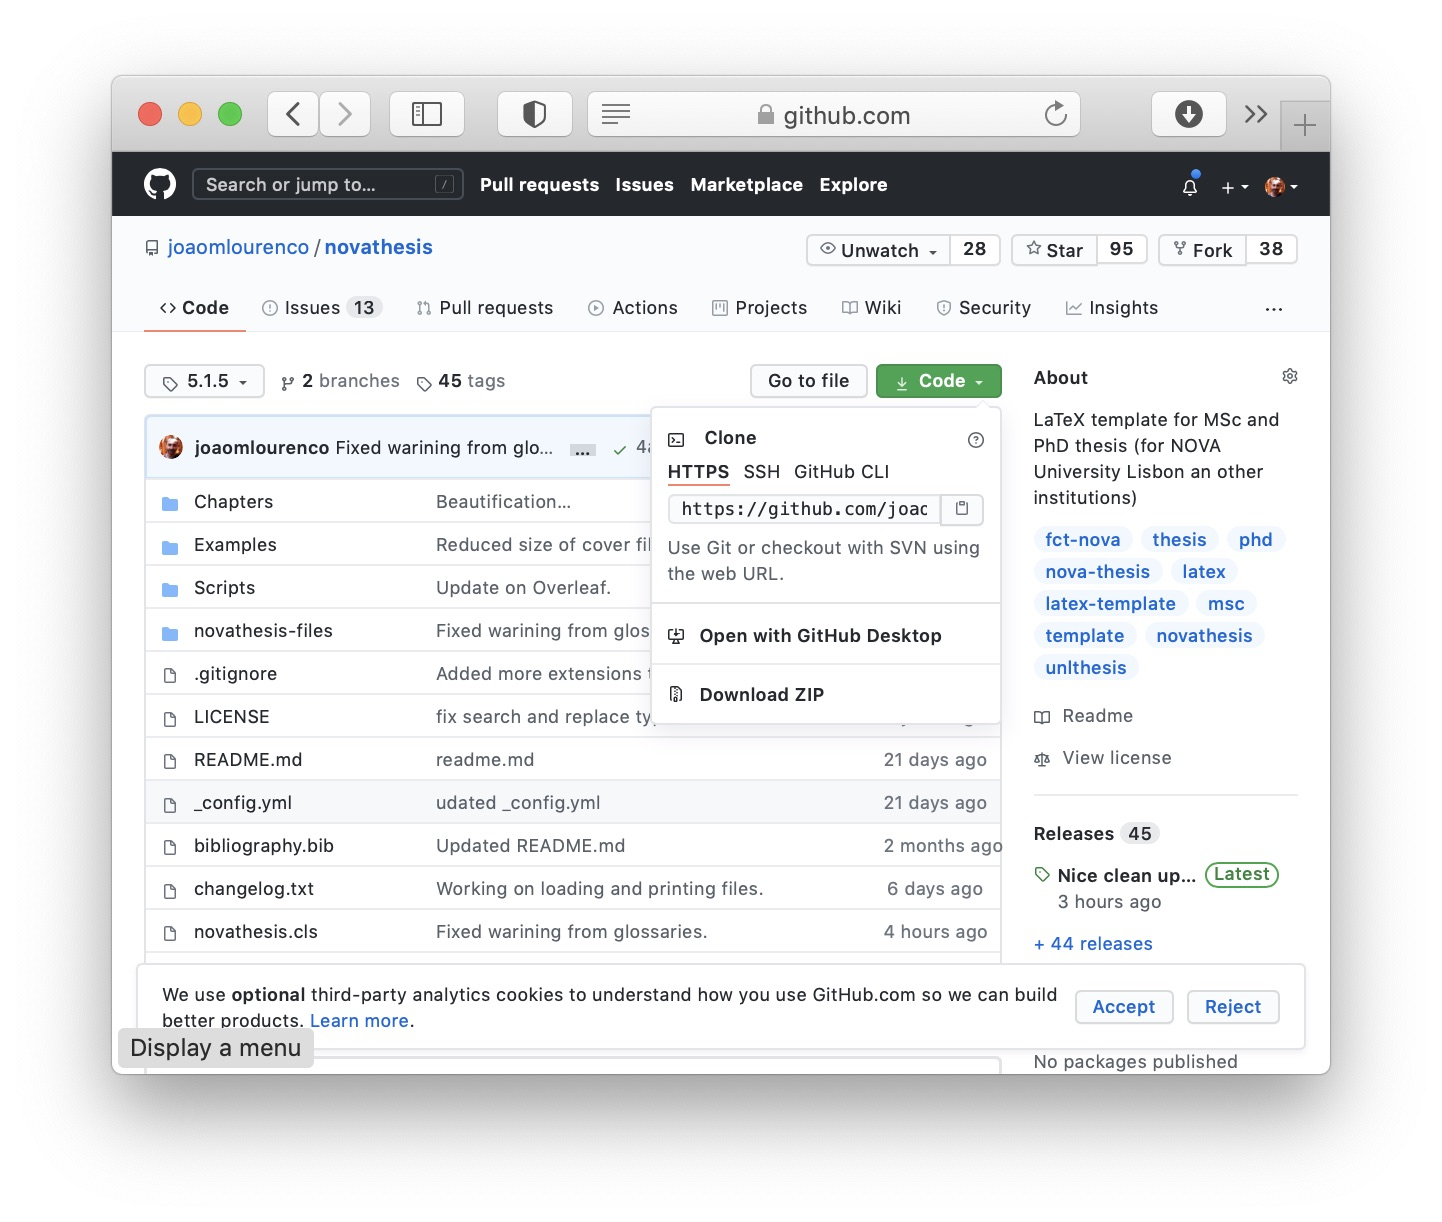
\includegraphics[width=\linewidth]{github}%
\caption{The NOVAthesis Project page in GitHub.}
\label{fig:github2}
\end{wrapfigure}

First of all, start by installing \LaTeX\ in your computer.  There are two main distributions, \href{https://miktex.org}{\ntindex{\MikTeX}}\ and \href{https://www.tug.org/texlive/}{\ntindex{\TeXLive}}, and both of them are available for the~3 most popular Operating Systems: Linux, macOS and Windows.

\section{Getting Help}
\label{sec:getting_help}

\ntindex[Help]{}

No! You don't have to use this template to write your thesis.  You don't even have to use \LaTeX.  However, writing a thesis is serious stuff, and which tool you shall use to write it is not a decision to make lighthearted.

\LaTeX\ is hard enough by itself.  This template aims at making your life easier, but not easy. If you choose to use this template to write your thesis, you are very welcome.  However, don't expect me to provide you help with \LaTeX.  Look for help with your friends (you have some friends, don't you?), or search the web, or try even to read some book(s) on \LaTeX. In the end you will certainly find the experience rewarding.

When you come to the point of “\emph{How do I do this with the \novathesis\ template?}”, remember…

\begin{enumerate}
  \item Search the \href{https://github.com/joaomlourenco/novathesis/discussions}{GitHub Discussions page} for a question related to yours.  \emph{If and only if} you don't find one, then post your own question in English please!
  \item Search the \href{https://www.facebook.com/groups/novathesis}{NOVAtheis Facebook group} for a question related to yours.  \emph{If and only if} you don't find one, then post your own question in either Portuguese or English, at your preference.
\end{enumerate}

\begin{tcolorbox}[colback=blue!8]
	\centering
Please do not attempt to contact me directly (email, Messenger, etc)…\\I WILL NOT REPLY!
\end{tcolorbox}

\subsection{Suggestions, Bugs and Feature Requests}
\begin{description}
  \item[Help:] If you just need some help, see above \Autoref{sec:getting_help}.
  \item[Suggestion:] \ntindex[Suggestions]{} Do you have a suggestion/recommendation? Please add it to the wiki and help other users!
  \item[Bug:] \ntindex[Bugs]{} Did you find a bug? Please open an issue. Thanks!
  \item[New Feature:] \ntindex[Feature Requests]{} Would you like to request a new feature (or support of a new School)? Please open an issue. Thanks!

\end{description}